\chapter{Introduzione}
\label{chap:introduzione}


%This is a reference to a chapter \ref{chap:quo}. This is a reference to a figure \ref{fig:doge}. This is a reference to some code \ref{lst:hello}. This is a citation \cite{famous:paper}.
%
%\lstinputlisting[label=lst:hello, firstline=2, lastline=4, caption={I directly included a portion of a file}]{code/hello.py}
%
%\begin{lstlisting}[language=Java, label=lst:java, caption={Some code in another language than the default one}]
%public void prepare(AClass foo) {
%        AnotherClass bar = new AnotherClass(foo)
%}
%\end{lstlisting}
%
%\Blindtext

Il panorama mondiale ha, nell'ultimo decennio, riposto particolare attenzione ed interesse verso le emergenti tecnologie nel campo dell'Internet of Things. \\ Questo perchè, il paradigma IoT consente oggi di realizzare la vision ed il concept che era già stato supposto e predetto come sviluppo della rete Internet. Ovvero adempiere allo scopo di collegare il mondo. \\
Tuttavia, se grazie ad Interent è stato possibile collegare le persone, metterle in relazione, fornire ad essi gli strumenti per interagire tra loro, indipendentemente dalla loro posizione geografica o razza o sesso o colore, allo stesso modo, il naturale sviluppo di Internet non può che essere quello di mettere in relazione le cose. I dispositivi che siamo abituati ad utilizzare ogni giorno e che, seppur diversi ed eterogenei tra loro in termini di funzionalità, costo e posizione, sono in grado di comunicare tra loro, scambiarsi dati ed informazioni al fine di cambiare definitivamente il nostro modo di lavorare, acquistare, consumare e quindi di vivere.
\begin{figure}
\begin{center}
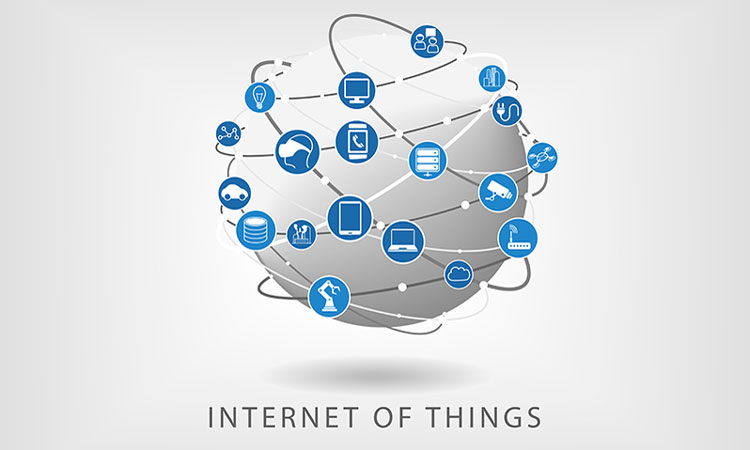
\includegraphics[width=0.7\columnwidth]{images/iot.jpg}
\end{center}
\caption{Overview del paradigma IoT}
\label{fig:iot}
\end{figure}

\section{IoT Enabling Technologies}
\label{sec:iot_enabling_technologies}

L'idea di una rete Internet che consentisse la comunicazione a livello globale tra persone o tra persone e cose o tra cose era già da molto tempo una visione condivsa di quello che sarebbe potuto essere lo sviluppo di Internet. \\
Tale visione è oggi possibile grazie alla diffusione capillare in qualsiasi strumento di piccoli, economici e potenti dispositivi di calcolo. \\
Tuttavia, affinchè una simile rivoluzione tecnologia si paventasse, era necessario superare i tradizionali protocolli di comunicazione tipici della rete Internet e creare conseguentemente delle nuove tecnologie per la comunicazione che fossero ottimizzate per le nuove esigenze.
Va infatti ricordato ancora una volta che la vision dell'IoT sia quella di abilitare una comunicazione tra qualsiasi tipo di dispositivo che abbia al suo interno una unità di calcolo. Questo significa stabilire una comunicazione tra dispositivi eterogenei, dispositivi che assolvono diversi compiti ed adempiono a diverse necessità e che sono molto spesso anche dotati di una diversa e limitata potenza di elaborazione. \\
Di qui la necessità di nuovi protocolli e tecnologie di comunicazione che non solo garantissero la comunicazione sicura di una grossa mole di dati tra un grande numero di dispositivi, ma che fossero anche dei protocolli leggeri dal punto di vista computazionale ed ovviamente economici, così da poter essere integrati in qualsiasi dispositivo, da quelli destinati all'industria a quelli destinati al mercato consumer.
Data la complessità della sfida tecnologica da fronteggiare e considerata l'eterogeneità del problema e delle necessità nei diversi campi applicativi,
sono stati sviluppati e proposti diverse tipologie di tecnologie e protocolli di comunicazione. \\
Tra le più rilevanti nel campo della comunicazione domestica o locale emergono Bluetooth Low Energy \cite{famous:paper_1} and Zigbee \cite{famous:paper_2}. Mentre altri protocolli come WiFi, LowPower Wide Area Networks (LPWA) \cite{famous:paper_3} e le comunicazioni cellulari come 3GPP , 4G o 5G \cite{famous:paper_Grieco_1} hanno uno scope più ampio, abilitando la comunicazione tra dispositivi anche molto distanti tra loro.


